\documentclass[conference]{IEEEtran}
\IEEEoverridecommandlockouts

\usepackage{amsmath,amssymb,amsfonts}
\usepackage{textcomp}
\usepackage{xcolor}
\usepackage{graphicx}
\usepackage{booktabs}
\usepackage{cite}
\usepackage{tikz}
\usetikzlibrary{shapes.geometric, arrows.meta, positioning, calc}
\usepackage{pgfplots}
\pgfplotsset{compat=1.18}

\def\BibTeX{{\rm B\kern-.05em{\sc i\kern-.025em b}\kern-.08em
    T\kern-.1667em\lower.7ex\hbox{E}\kern-.125emX}}

\begin{document}

\title{Auditing the Reliability of LLM-Generated Testbenches for Verilog RTL Verification}

\author{\IEEEauthorblockN{Soham Guha}
\IEEEauthorblockA{\textit{School of Computer Engineering} \\
\textit{Kalinga Institute of Industrial Technology (KIIT) Deemed to be University}\\
Bhubaneswar, Odisha, India \\
Email: soham.guha@kiit.ac.in}
}

\maketitle

\begin{abstract}
Large language models (LLMs) are increasingly applied to automate hardware register-transfer level (RTL) design synthesis. However, the integrity of automated hardware design depends on the reliability of the verification artifacts used to evaluate candidate circuits. In hardware verification, an incorrect testbench that rejects a correct design creates a \textit{false rejection}, misdirecting automated iteration loops and squandering expensive engineering or compute cycles. This paper presents an empirical audit of the reliability of LLM-generated Verilog testbenches across 1,022 free-form generation trials evaluated on 30 benchmark problems from the VerilogEval-v2 benchmark suite. In our evaluation corpus, 58.32\% of all trials (596 of 1,022; 95\% Wilson CI [55.27\%, 61.30\%]; problem-level cluster bootstrap 95\% CI [48.37\%, 67.70\%]) constitute false rejections: the testbench compiles cleanly and meets output interface contracts, but nonetheless fails when simulated against the golden reference design. Conditioning on syntactically valid and contract-compliant testbenches increases the observed failure rate to 61.25\% (596 of 973; cluster bootstrap CI [52.31\%, 69.54\%]). We investigate whether false rejections can be mitigated through adversarial setups, including same-family and cross-family second-model checkers, specification-only visibility, and compute-matched controls. Observed false-rejection rates remain between 54\% and 62\% across all six evaluated conditions, and neither an omnibus Pearson chi-square test ($\chi^2 = 4.36, p = 0.499$) nor a problem-level paired permutation test ($p = 0.144$) indicates statistically significant differences among conditions. Furthermore, audit of the benchmark specifications reveals that while specification ambiguities and reference mismatches account for a subset of failures, false rejections persist even on clean, combinational problems (12.33\% to 24.77\%). Finally, a paired problem-level comparison between GPT-4o-mini and Gemini Flash-Lite indicates a statistically significant difference in per-problem false-rejection rate (-10.47 percentage points; 95\% bootstrap CI [-16.88\%, -4.27\%]). We discuss methodological limits, including the reliance on single-engine simulation and unverified golden reference oracles.
\end{abstract}

\begin{IEEEkeywords}
Hardware Verification, Large Language Models, Verilog RTL, Testbench Synthesis, False Rejection, Empirical Software Engineering.
\end{IEEEkeywords}

\section{Introduction}
Recent progress in large language models (LLMs) has motivated their application across electronic design automation (EDA), specifically targeting register-transfer level (RTL) synthesis in languages such as Verilog~\cite{liu2023verilogeval, lu2024rtllm, blocklove2023chipchat}. Frameworks such as AutoChip~\cite{thakur2023autochip} propose closing the loop by using LLMs not only to author candidate hardware modules, but also to generate accompanying testbenches and parse simulation feedback autonomously.

In traditional software development, a flawed test may cause a transient regression failure in a continuous integration environment. In hardware engineering, however, verification holds a distinct and unforgiving role~\cite{wile2005verilog}. Pre-silicon functional bugs that escape detection lead to catastrophic mask refabrication costs or field recalls. Conversely, a flawed verification harness that falsely flags a correct implementation---termed here a \textit{false rejection}---misdirects synthesis engines, causes spurious repair loops, and invalidates claims of autonomous design capability.

Despite substantial research evaluating LLMs on RTL code generation~\cite{liu2023verilogeval, lu2024rtllm}, the reliability of LLM-generated \textit{testbenches} has received comparatively limited empirical scrutiny. Standard evaluation protocols frequently assume an asymmetric reliability model: candidate designs are treated as untrusted, while LLM-synthesized verification harnesses or multi-agent debate protocols are presumed capable of serving as reliable oracles~\cite{du2023debate}. If the testbench itself systematically misinterprets interface timing, misapprehends reset semantics, or asserts incorrect output values, downstream verification decisions become untrustworthy.

To evaluate this concern, we conducted a controlled empirical audit of LLM-synthesized Verilog testbenches. We examine 1,022 free-form generation trials across 30 specification-to-RTL benchmark problems derived from VerilogEval-v2~\cite{liu2023verilogeval,pinckney2024revisiting}. Our experimental pipeline subjects each generated testbench to three sequential validation gates:
\begin{enumerate}
    \item \textit{Gate 1 (Compilation and Contract Compliance):} The testbench must compile under Icarus Verilog 12.0 (\texttt{-g2012}) and adhere to the prescribed simulation output format without runtime syntax failures.
    \item \textit{Gate 2 (Golden Reference Simulation):} The testbench must pass when simulated against the official golden reference RTL implementation.
    \item \textit{Gate 3 (Non-Vacuity Gate):} The testbench must reject a known-defective mutated circuit (an inverted-output design) to confirm that its pass condition is non-vacuous.
\end{enumerate}

A trial is formally classified as a \textit{false rejection} ($F_i$) when it successfully compiles and complies with output contracts, yet fails the simulation on the golden reference design:
\begin{equation}
F_i = C_i \land K_i \land \neg G_i
\label{eq:fr_def}
\end{equation}
where $C_i$ indicates successful compilation, $K_i$ indicates contract validity, and $G_i$ indicates passing the golden RTL simulation.

This audit addresses four central research questions:
\begin{itemize}
    \item \textbf{RQ1 (Prevalence):} What proportion of LLM-generated testbenches falsely reject the golden reference design?
    \item \textbf{RQ2 (Condition Invariance):} Do adversarial, cross-family, or specification-only prompting structures reduce the rate of false rejections compared to self-testing baselines?
    \item \textbf{RQ3 (Circuit Complexity and Specification Ambiguity):} How do false-rejection rates vary across combinational versus sequential circuits, and to what degree are failures attributable to specification defects rather than model hallucinations?
    \item \textbf{RQ4 (Model Sensitivity):} Does false-rejection susceptibility differ systematically across distinct commercial LLM families when compared over identical problem cohorts?
\end{itemize}

Our empirical findings reveal that false rejection is not an isolated edge case, but the predominant failure mode in our testbench generation trials, with an overall rate of 58.32\% across all trials (61.25\% among syntactically valid and contract-compliant testbenches). Across six evaluated generation conditions, observed failure rates remained consistently between 54\% and 62\%, showing no statistically significant mitigation from cross-family adversarial setups or compute matching. While specification defects and sequential reset ambiguities contribute substantially to these failures, a persistent residual error rate remains even on unambiguous combinational designs.

\section{Related Work}
\subsection{LLMs in RTL Generation and Verification}
The benchmark suites VerilogEval~\cite{liu2023verilogeval} and RTLLM~\cite{lu2024rtllm} standardized the evaluation of generative models on Verilog synthesis tasks. These benchmarks demonstrated that frontier models can synthesize simple arithmetic modules, state machines, and interface logic. However, functional verification within these benchmark suites relies on fixed, hand-crafted reference testbenches developed by human authors.


Efforts to automate the verification side of the flow have explored generating SystemVerilog assertions (SVA) from natural language specifications~\cite{yan2025assertllm} and using LLMs in conversational feedback loops (e.g., Chip-Chat~\cite{blocklove2023chipchat} and AutoChip~\cite{thakur2023autochip}). In AutoChip, LLM-generated code is simulated against an execution harness, and simulation compiler errors or test assertions are fed back to the model for iterative refinement. Closest to our setting, AutoBench~\cite{qiu2024autobench} and CorrectBench~\cite{qiu2024correctbench} generate testbenches with LLMs and score them against golden RTL and RTL mutants; CorrectBench adds functional self-validation and self-correction. Our audit instead isolates false rejection of the golden design and tests cross-family adversarial checking. However, AutoChip assumes that the simulation oracle correctly reflects the true specification. If the verification harness is itself synthesized by an LLM, any bias or misunderstanding in the generated testbench risks corrupting the feedback signal.

\subsection{Multi-Agent Consensus and Adversarial Verification}
To address hallucination in generative models, prior software engineering and reasoning literature has proposed multi-agent debate and consensus voting~\cite{du2023debate}. In hardware, proposals have suggested pairing a generator model from one family (e.g., OpenAI GPT) with an adversarial verifier from another family (e.g., Anthropic Claude or Google Gemini) to eliminate correlated blind spots. The underlying hypothesis posits that models trained on distinct corpora and utilizing different tokenization architectures will not make identical errors when interpreting hardware timing specifications. We explicitly evaluate this hypothesis by comparing self-testing against same-family and cross-family adversaries under controlled compute allocations.

\section{Experimental Methodology}

\begin{figure*}[t]
\centering
\resizebox{\textwidth}{!}{%
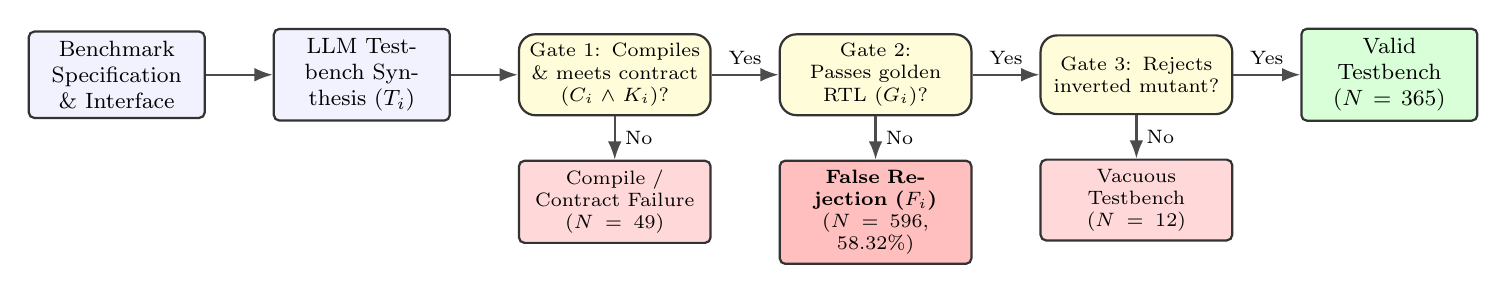
\begin{tikzpicture}[
    node distance=0.55cm and 0.85cm,
    box/.style={rectangle, draw=black!80, fill=blue!5, thick, rounded corners=2pt, text width=2.0cm, minimum height=1.0cm, align=center, font=\footnotesize},
    gate/.style={rectangle, draw=black!80, fill=yellow!15, thick, rounded corners=6pt, text width=2.2cm, minimum height=1.0cm, align=center, font=\scriptsize},
    term/.style={rectangle, draw=black!80, fill=red!15, thick, rounded corners=2pt, text width=2.2cm, minimum height=0.9cm, align=center, font=\scriptsize},
    pass/.style={rectangle, draw=black!80, fill=green!15, thick, rounded corners=2pt, text width=2.0cm, minimum height=1.0cm, align=center, font=\footnotesize},
    arrow/.style={-Latex, thick, draw=black!70}
]

\node[box]  (spec) {Benchmark Specification \& Interface};
\node[box, right=of spec] (gen) {LLM Testbench Synthesis ($T_i$)};
\node[gate, right=of gen] (g1) {Gate 1: Compiles \& meets contract ($C_i \land K_i$)?};
\node[gate, right=of g1]  (g2) {Gate 2: Passes golden RTL ($G_i$)?};
\node[gate, right=of g2]  (g3) {Gate 3: Rejects inverted mutant?};
\node[pass, right=of g3]  (valid) {Valid Testbench\\($N=365$)};

\node[term, below=of g1] (fail_g1) {Compile / Contract Failure\\($N=49$)};
\node[term, below=of g2, fill=red!25] (fr) {\textbf{False Rejection ($F_i$)}\\($N=596$, 58.32\%)};
\node[term, below=of g3] (vac) {Vacuous Testbench\\($N=12$)};

\draw[arrow] (spec) -- (gen);
\draw[arrow] (gen) -- (g1);
\draw[arrow] (g1) -- node[above, font=\scriptsize] {Yes} (g2);
\draw[arrow] (g1) -- node[right, font=\scriptsize] {No} (fail_g1);
\draw[arrow] (g2) -- node[above, font=\scriptsize] {Yes} (g3);
\draw[arrow] (g2) -- node[right, font=\scriptsize] {No} (fr);
\draw[arrow] (g3) -- node[above, font=\scriptsize] {Yes} (valid);
\draw[arrow] (g3) -- node[right, font=\scriptsize] {No} (vac);

\end{tikzpicture}%
}
\caption{Three-gate testbench validation pipeline. A generated testbench is categorized as a false rejection ($F_i$) if it successfully compiles and conforms to output contracts at Gate 1, but fails simulation against the golden reference RTL at Gate 2.}
\label{fig:pipeline}
\end{figure*}

\subsection{Benchmark Problem Suite}
Our evaluation dataset consists of 30 benchmark problems drawn from the VerilogEval-v2 spec-to-RTL problem suite~\cite{liu2023verilogeval}. The problems span basic building blocks: 8 combinational circuits (including vector operations, multiplexers, and arithmetic priority encoders) and 22 sequential circuits (including binary counters, LFSRs, shift registers, and finite state machines). Trivial single-gate assignments were omitted. 

Each problem in the repository includes:
\begin{itemize}
    \item A natural language functional specification (\texttt{spec.txt}).
    \item A golden reference RTL implementation (\texttt{ref.v}).
    \item An official reference testbench (\texttt{tb.v}) providing known stimulus vectors.
\end{itemize}

\subsection{Execution Environment and Tooling}
Simulations were executed natively using Icarus Verilog version 12.0 (devel) with SystemVerilog-2012 extensions enabled (\texttt{iverilog -g2012}). Simulation runtimes were constrained by a strict timeout (15 seconds) to prevent infinite loops from malformed testbench clocks. 

We investigated deploying Verilator (version 5.032) as an independent secondary simulation compiler. However, the official benchmark verification harnesses and LLM-generated testbenches make extensive use of delayed assignment constructs (\texttt{\#5}, \texttt{\#10}), event control statements (\texttt{@(posedge clk)}), and initial blocks that are not synthesizable and cannot be compiled by Verilator's cycle-based engine without extensive testbench restructuring. As a consequence, multi-simulator consensus could not be supported, and all simulation results reported herein rely on Icarus Verilog.

\subsection{Experimental Arms and Archival Structure}
The complete archived repository contains 1,112 total experimental trials across two distinct arms:
\begin{enumerate}
    \item \textit{Template-Pilot Arm ($N=90$):} A pilot study where the verification harness provided a fixed SystemVerilog template containing clock generators, reset pulses, and module instantiation scaffolds, requiring the model only to populate input stimuli. In this arm, 75 of 90 trials failed to compile due to syntax and out-of-scope procedural statements, and the remaining 15 were vacuous. None achieved false-rejection status because none passed Gate 1. This arm was excluded from primary quantitative analysis.
    \item \textit{Free-Form Generation Arm ($N=1,022$):} The primary evaluation corpus, wherein language models autonomously author complete, standalone self-checking Verilog testbenches given the specification and interface declarations.
\end{enumerate}

Trials were collected across pseudo-random generator seeds 42, 43, and 44 with model generation temperature fixed at 0.20 to balance syntactic determinism with sampling diversity. Total trials per problem range from 18 to 54 depending on problem inclusion across experimental iterations.

\subsection{Experimental Conditions}
To rigorously assess whether adversarial or multi-agent configurations alleviate verification failure, the 1,022 free-form trials were partitioned into six distinct experimental conditions:
\begin{itemize}
    \item \textbf{Condition A (Self-Test Baseline, $n=171$):} The generator model $G$ authors candidate RTL, and the same model $G$ synthesizes the testbench with visibility of both the specification and candidate RTL.
    \item \textbf{Condition B (Same-Family Adversary, $n=170$):} A second model $G'$ from the same model family synthesizes the testbench with visibility of both the specification and candidate RTL.
    \item \textbf{Condition B' (Same-Family Spec-Only, $n=170$):} Model $G'$ synthesizes the testbench given the specification only; the candidate RTL is hidden to prevent anchoring bias.
    \item \textbf{Condition C (Cross-Family Adversary, $n=170$):} An adversarial model $T$ from a distinct architectural family synthesizes the testbench with visibility of specification and candidate RTL.
    \item \textbf{Condition C' (Cross-Family Spec-Only, $n=170$):} Model $T$ synthesizes the testbench given the specification only; the candidate RTL is hidden.
    \item \textbf{Condition D (Compute-Matched Self-Test, $n=171$):} The generator model $G$ tests its own design, but is allocated a doubled sampling and retry token budget matched to the aggregate compute expended in Condition C.
\end{itemize}

\subsection{Evaluation Pipeline and Gates}
As illustrated in Fig.~\ref{fig:pipeline}, every synthesized testbench is processed through three sequential gates:
\begin{itemize}
    \item \textbf{Gate 1: Compilation and Contract Validation ($C_i \land K_i$):} The testbench is compiled alongside the reference design. It must produce an executable binary without syntax errors ($C_i = 1$) and print standardized status messages (\texttt{*** TEST RESULT: PASS ***} or \texttt{FAIL}) complying with parsing rules ($K_i = 1$).
    \item \textbf{Gate 2: Simulation Against Golden RTL ($G_i$):} The compiled binary is executed. If the testbench asserts a mismatch or terminates with a failure status on the golden reference design, $G_i = 0$.
    \item \textbf{Gate 3: Inverted Output Non-Vacuity Gate:} If a testbench reports a pass on the golden RTL, it is simulated against an artificially inverted circuit mutant. If the testbench still reports \texttt{PASS} on the inverted mutant, it is flagged as vacuous and rejected.
\end{itemize}
A trial is confirmed as a false rejection ($F_i = 1$) if and only if $C_i = 1$, $K_i = 1$, and $G_i = 0$.

\subsection{Model Allocation}
The free-form trials in the archival dataset incorporate three model configurations acting as generators and testers:
\begin{itemize}
    \item \textbf{GPT-4o-mini (\texttt{gpt-4o-mini-2024-07-18}):} Evaluated across 540 generation trials and 514 testbench synthesis trials across all 30 problems.
    \item \textbf{Gemini Flash-Lite (\texttt{gemini-3.5-flash-lite}):} Evaluated across 462 generation trials and 488 testbench synthesis trials spanning 26 of the 30 problems.
    \item \textbf{Qwen2.5-Coder-1.5B (\texttt{qwen2.5-coder:1.5b}):} Evaluated across 20 trials on 2 pilot benchmark problems (\texttt{Prob035} and \texttt{Prob040}).
\end{itemize}

\subsection{Statistical Methods and Clustering}
Trials in our dataset are grouped within 30 benchmark problems. Because multiple trials evaluate the same underlying Verilog module, observations within the same problem cluster exhibit statistical dependence. 

Analysis of variance reveals an intraclass correlation coefficient (ICC) of $\rho \approx 0.2665$ across the 30 problem clusters. With an average cluster size of $\bar{m} = 34.07$ trials per problem, the design effect is:
\begin{equation}
D_{\text{eff}} = 1 + (\bar{m} - 1)\rho \approx 1 + (33.07)(0.2665) \approx 9.81
\end{equation}
This design effect indicates that standard variance estimators treating observations as independent overstate statistical precision by nearly an order of magnitude, yielding an effective sample size of $n_{\text{eff}} = N / D_{\text{eff}} \approx 1022 / 9.81 \approx 104.1$.

Accordingly, while we report standard Wilson score intervals~\cite{wilson1927probable} for unadjusted trial-level proportions, our primary inferential intervals are computed using a problem-level cluster bootstrap~\cite{cameron2015practitioner, efron1994introduction}. Specifically, we draw 10,000 bootstrap resamples with replacement at the problem level (resampling entire problem clusters), recomputing rates over all trials contained in the resampled clusters using a fixed random seed of 42.

\section{Empirical Results}

\begin{table*}[t]
\centering
\caption{False Rejection Rates Across Benchmark Subsets (Seed 42, 10,000 Bootstrap Draws)}
\label{tab:headline_rates}
\footnotesize
\setlength{\tabcolsep}{4pt}
\begin{tabular}{lcccccc}
\toprule
\textbf{Evaluation Subset} & \textbf{Problems} & \textbf{Trials ($N$)} & \textbf{$F_i$} & \textbf{Rate (\%)} & \textbf{Wilson 95\% CI} & \textbf{Cluster Bootstrap 95\% CI} \\
\midrule
All Trials (Unconditional) & 30 & 1,022 & 596 & \textbf{58.32} & [55.27, 61.30] & [48.37, 67.70] \\
Conditional ($C_i \land K_i$) & 30 & 973 & 596 & \textbf{61.25} & [58.15, 64.26] & [52.31, 69.54] \\
\midrule
Excl. 3 Inconsistent Problems & 27 & 914 & 505 & \textbf{55.25} & [52.01, 58.45] & [45.28, 64.94] \\
Excl. Inconsistent (Conditional) & 27 & 868 & 505 & \textbf{58.18} & [54.87, 61.42] & [49.16, 66.48] \\
\midrule
Combinational (All) & 8 & 290 & 98 & \textbf{33.79} & [28.59, 39.42] & [17.83, 49.66] \\
Combinational (Conditional) & 8 & 243 & 98 & \textbf{40.33} & [34.36, 46.60] & [23.36, 54.98] \\
Sequential (All) & 22 & 732 & 498 & \textbf{68.03} & [64.57, 71.31] & [58.99, 76.23] \\
Sequential (Conditional) & 22 & 730 & 498 & \textbf{68.22} & [64.75, 71.49] & [59.10, 76.53] \\
\midrule
6 Clean Combinational (Post-hoc) & 6 & 218 & 54 & \textbf{24.77} & [19.51, 30.90] & [9.68, 40.60] \\
6 Clean Combinational (Conditional) & 6 & 177 & 54 & \textbf{30.51} & [24.20, 37.65] & [13.51, 45.02] \\
4 Simple Combinational (Post-hoc) & 4 & 146 & 18 & \textbf{12.33} & [7.94, 18.65] & [1.79, 18.89] \\
4 Simple Combinational (Conditional) & 4 & 108 & 18 & \textbf{16.67} & [10.81, 24.81] & [2.63, 24.29] \\
\bottomrule
\end{tabular}
\end{table*}

\subsection{RQ1: Overall False Rejection Incidence}
Across all 1,022 free-form generation trials, 973 trials (95.20\%) successfully compiled and conformed to simulation contracts (Gate 1). However, only 377 trials passed the simulation on the golden reference RTL design. Among the remaining trials, 12 testbenches were flagged as vacuous at Gate 3. 

In total, 596 trials satisfied $C_i \land K_i \land \neg G_i$, yielding an overall false-rejection rate of:
\begin{equation}
\text{FRR}_{\text{all}} = \frac{596}{1,022} = 58.32\% \quad (\text{Wilson: } [55.27\%, 61.30\%])
\end{equation}
When clustered by problem design, the 95\% cluster bootstrap confidence interval is [48.37\%, 67.70\%].

When evaluating only the testbenches that successfully satisfied Gate 1 ($N=973$), the conditional false-rejection rate rises to:
\begin{equation}
\text{FRR}_{\text{cond}} = \frac{596}{973} = 61.25\% \quad (\text{Wilson: } [58.15\%, 64.26\%])
\end{equation}
with a problem-level cluster bootstrap 95\% CI of [52.31\%, 69.54\%].

To verify data integrity, we recomputed the false-rejection flag directly from raw simulator standard output (\texttt{golden\_sim\_stdout}) and contract fields across all 1,022 trials, observing 0 discrepancies. Furthermore, in an independent physical rerun of 85 sampled false-rejection trials under Icarus Verilog 12.0, all 85 trials (100\%) reproduced their exact failure assertions.

\subsection{RQ2: Impact of Prompting Conditions and Adversaries}
Table~\ref{tab:conditions} details false-rejection rates across the six experimental conditions. Observed false-rejection rates remain within a narrow band between 54\% and 62\% across all arms:
\begin{itemize}
    \item Condition A (Self-Test): 93 of 171 (54.39\%, Wilson [46.91\%, 61.67\%])
    \item Condition B (Same-Family + RTL): 106 of 170 (62.35\%, Wilson [54.87\%, 69.29\%])
    \item Condition B' (Same-Family Spec-Only): 104 of 170 (61.18\%, Wilson [53.68\%, 68.18\%])
    \item Condition C (Cross-Family + RTL): 97 of 170 (57.06\%, Wilson [49.54\%, 64.26\%])
    \item Condition C' (Cross-Family Spec-Only): 103 of 170 (60.59\%, Wilson [53.09\%, 67.62\%])
    \item Condition D (Compute-Matched Control): 93 of 171 (54.39\%, Wilson [46.91\%, 61.67\%])
\end{itemize}

An omnibus Pearson chi-square test~\cite{pearson1900criterion} on the $2 \times 6$ contingency table of outcomes yields:
\begin{equation}
\chi^2 = 4.3566, \quad df = 5, \quad p = 0.4993
\end{equation}
indicating no statistically significant variation in false-rejection rate across conditions.

To evaluate whether pairing models introduces subtle benefits masked by pooling, we performed a cluster-aware, problem-level paired permutation test comparing Condition B to Condition A. For each of the 30 problems, we computed the per-problem rate difference $\Delta_p = \text{Rate}_B(p) - \text{Rate}_A(p)$. Across problems, Condition B exhibited a higher observed mean false-rejection rate ($+7.78$ percentage points). Under 10,000 paired sign-flip permutation draws with seed 42, this difference yields a two-sided permutation $p$-value of $p = 0.1436$.

Because neither the omnibus chi-square test nor the paired permutation test achieves statistical significance, the empirical data does not support ranking or distinguishing the prompting conditions.

\begin{table}[t]
\centering
\caption{Outcome Breakdown Across Experimental Conditions}
\label{tab:conditions}
\footnotesize
\setlength{\tabcolsep}{3pt}
\begin{tabular}{lcccrc}
\toprule
\textbf{Cond.} & \textbf{$N$} & \textbf{Pass G1} & \textbf{$F_i$} & \textbf{Rate (\%)} & \textbf{Wilson 95\% CI} \\
\midrule
A (Self)         & 171 & 158 & 93  & 54.39 & [46.91, 61.67] \\
B (Same+RTL)     & 170 & 162 & 106 & 62.35 & [54.87, 69.29] \\
B$'$ (Same-Spec) & 170 & 166 & 104 & 61.18 & [53.68, 68.18] \\
C (Cross+RTL)    & 170 & 160 & 97  & 57.06 & [49.54, 64.26] \\
C$'$ (Cross-Spec)& 170 & 166 & 103 & 60.59 & [53.09, 67.62] \\
D (Matched)      & 171 & 161 & 93  & 54.39 & [46.91, 61.67] \\
\bottomrule
\end{tabular}

\vspace{3pt}
\begin{minipage}{0.96\columnwidth}
\scriptsize
Pearson $\chi^2 = 4.3566$, $df = 5$, $p = 0.4993$ (not significant). Problem-level paired permutation (B vs.\ A): diff $= +7.78$ pp, $p = 0.1436$.
\end{minipage}
\end{table}

\subsection{RQ3: Circuit Complexity and Specification Quality}
\subsubsection{Combinational vs. Sequential Complexity}
As shown in Table~\ref{tab:headline_rates}, false rejections are strongly stratified by circuit category:
\begin{itemize}
    \item \textit{Combinational Circuits (8 problems, $N=290$):} 98 false rejections, yielding an all-trials rate of 33.79\% (cluster bootstrap CI [17.83\%, 49.66\%]) and a conditional rate of 40.33\% (cluster CI [23.36\%, 54.98\%]).
    \item \textit{Sequential Circuits (22 problems, $N=732$):} 498 false rejections, yielding an all-trials rate of 68.03\% (cluster bootstrap CI [58.99\%, 76.23\%]) and a conditional rate of 68.22\% (cluster CI [59.10\%, 76.53\%]).
\end{itemize}

\subsubsection{Impact of Verified Specification Inconsistencies}
A systematic audit of specification texts against reference RTL code revealed three problems containing explicit, irreconcilable contradictions:
\begin{enumerate}
    \item \texttt{Prob068\_countbcd}: Specification defines enable signal \texttt{ena} as 4 bits (\texttt{[3:0]}), whereas the golden reference RTL declares \texttt{[3:1]} (3 bits).
    \item \texttt{Prob088\_ece241\_2014\_q5b}: Specification explicitly demands a one-hot state assignment, whereas reference RTL implements binary sequential state parameters.
    \item \texttt{Prob099\_m2014\_q6c}: Specification declares a 7-bit bus, whereas reference RTL implements 6 bits; specification text refers to signals \texttt{Y2} and \texttt{Y4} while module ports declare \texttt{Y1} and \texttt{Y3}.
\end{enumerate}
Across these three problems (108 trials), 91 trials resulted in false rejections. Excluding these three problems reduces the overall dataset from 1,022 to 914 trials across 27 problems. On this pruned subset:
\begin{itemize}
    \item All-trials rate: 505 of 914 = 55.25\% (cluster bootstrap CI [45.28\%, 64.94\%]).
    \item Conditional rate: 505 of 868 = 58.18\% (cluster bootstrap CI [49.16\%, 66.48\%]).
\end{itemize}
While specification defects account for 91 failures, their removal reduces the overall failure rate by only 3.07 percentage points.

\subsubsection{Exploratory Analysis of Clean Combinational Designs}
To evaluate whether false rejections can be eliminated under pristine specification conditions, we performed an exploratory post-hoc partition of the combinational benchmark suite. 

Six combinational problems satisfied strict specification audit criteria: \texttt{Prob006\_vectorr}, \texttt{Prob021\_mux256to1v}, \texttt{Prob033\_ece241\_2014\_q1c}, \texttt{Prob091\_2012\_q2b}, \texttt{Prob100\_fsm3comb}, and \texttt{Prob114\_bugs\_case}. On these 6 problems ($N=218$), the false-rejection rate is 24.77\% (54 of 218; cluster bootstrap CI [9.68\%, 40.60\%]). 

Two of these problems (\texttt{Prob091} and \texttt{Prob100}) specify next-state transition logic for finite state machines, where models frequently introduced unprompted sequential register or clocking assumptions. Excluding these two transition problems isolates four strictly combinational modules (\texttt{Prob006}, \texttt{Prob021}, \texttt{Prob033}, and \texttt{Prob114}, $N=146$). On this subgroup:
\begin{itemize}
    \item All-trials rate: 18 of 146 = 12.33\% (cluster bootstrap CI [1.79\%, 18.89\%]).
    \item Conditional rate: 18 of 108 = 16.67\% (cluster bootstrap CI [2.63\%, 24.29\%]).
\end{itemize}
Even when specifications are unambiguous and circuits lack sequential state, a non-zero baseline of false rejections persists.

\begin{figure}[t]
\centering
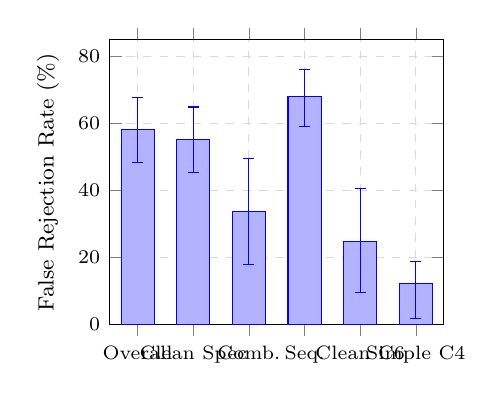
\begin{tikzpicture}
\begin{axis}[
    ybar,
    bar width=12pt,
    width=0.48\textwidth,
    height=5.2cm,
    ymin=0,
    ymax=85,
    ylabel={False Rejection Rate (\%)},
    symbolic x coords={All, Excl-Incon, Comb, Seq, Clean-Comb, Simple-4},
    xtick=data,
    xticklabels={Overall, Clean Spec, Comb., Seq., Clean C6, Simple C4},
    x tick label style={font=\scriptsize, align=center},
    y tick label style={font=\scriptsize},
    ylabel style={font=\footnotesize},
    grid=major,
    grid style={dashed, gray!30},
    legend style={at={(0.5,1.05)}, anchor=south, legend columns=2, font=\scriptsize}
]

\addplot+[error bars/.cd, y dir=both, y explicit]
coordinates {
    (All, 58.32)        += (0, 9.38)  -= (0, 9.95)
    (Excl-Incon, 55.25) += (0, 9.69)  -= (0, 9.97)
    (Comb, 33.79)       += (0, 15.87) -= (0, 15.96)
    (Seq, 68.03)        += (0, 8.20)  -= (0, 9.04)
    (Clean-Comb, 24.77) += (0, 15.83) -= (0, 15.09)
    (Simple-4, 12.33)   += (0, 6.56)  -= (0, 10.54)
};

\end{axis}
\end{tikzpicture}
\caption{False rejection rates across benchmark groupings with 95\% problem-level cluster bootstrap confidence intervals.}
\label{fig:rates_chart}
\end{figure}

\subsection{RQ4: Model Comparison}
Because model allocations in the archived dataset were not fully balanced across all 30 problems, we conducted fair, paired problem-level comparisons restricted to the shared problem cohorts.

\subsubsection{Primary Cohort (\texttt{generator\_id})}
Under the primary experimental assignment matching the 540 vs. 462 trial partition, both GPT-4o-mini and Gemini Flash-Lite evaluated an overlapping set of 26 problems (all problems except \texttt{Prob110}, \texttt{Prob111}, \texttt{Prob114}, and \texttt{Prob115}). On 25 problems, each model had 18 trials; on \texttt{Prob109}, GPT-4o-mini had 18 trials and Gemini Flash-Lite had 12.

As shown in Table~\ref{tab:model_comparison}, the mean per-problem false-rejection rate is 65.81\% for GPT-4o-mini and 55.34\% for Gemini Flash-Lite. The mean paired difference ($\Delta_p = \text{Rate}_{\text{Gemini}} - \text{Rate}_{\text{GPT}}$) is:
\begin{equation}
\bar{\Delta} = -10.47 \text{ pp} \quad (\text{95\% Bootstrap CI: } [-16.88\%, -4.27\%])
\end{equation}
Because the bootstrap confidence interval excludes zero, Gemini Flash-Lite exhibited a statistically significantly lower per-problem false-rejection rate across these 26 problems. Excluding the three inconsistent problems yields a consistent difference of $-10.63$ percentage points (95\% bootstrap CI $[-17.15\%, -4.35\%]$).

\subsubsection{Testbench Author Cohort (\texttt{tester\_id})}
If model roles are defined strictly by the model synthesizing the testbench (\texttt{tester\_id}), both models evaluated all 30 problems (514 trials for GPT-4o-mini, 488 trials for Gemini Flash-Lite). In this configuration:
\begin{itemize}
    \item GPT-4o-mini: 72.87\% mean per-problem FR rate.
    \item Gemini Flash-Lite: 41.64\% mean per-problem FR rate.
    \item Mean paired difference: $-31.23$ percentage points (95\% bootstrap CI $[-42.53\%, -20.48\%]$).
\end{itemize}
Excluding inconsistent problems yields a paired difference of $-32.03$ percentage points (95\% bootstrap CI $[-43.96\%, -20.84\%]$).

At the raw trial level across all 30 problems:
\begin{itemize}
    \item GPT-4o-mini authored testbenches failed on 382 of 514 trials (74.3\%, Wilson [70.4\%, 77.9\%]).
    \item Gemini Flash-Lite authored testbenches failed on 208 of 488 trials (42.6\%, Wilson [38.3\%, 47.1\%]).
    \item Llama-8b authored testbenches failed on 6 of 20 trials (30.0\%, Wilson [14.5\%, 51.9\%]).
\end{itemize}

\begin{table}[t]
\centering
\caption{Fair Paired Problem-Level Model Comparison (Seed 42, 10,000 Draws). GPT = GPT-4o-mini; Gemini = Gemini Flash-Lite; rates in \%, differences in percentage points (pp).}
\label{tab:model_comparison}
\footnotesize
\setlength{\tabcolsep}{3pt}
\begin{tabular}{lccrc}
\toprule
\textbf{Metric} & \textbf{GPT} & \textbf{Gemini} & \textbf{Diff. (pp)} & \textbf{95\% Boot. CI} \\
\midrule
\multicolumn{5}{l}{\textit{Generator cohort (\texttt{generator\_id}), 26 problems}} \\
Mean problem rate     & 65.81 & 55.34 & $-10.47$ & [$-16.88$, $-4.27$] \\
Excl. inconsistent (23) & 62.80 & 52.17 & $-10.63$ & [$-17.15$, $-4.35$] \\
\midrule
\multicolumn{5}{l}{\textit{Tester cohort (\texttt{tester\_id}), 30 problems}} \\
Mean problem rate     & 72.87 & 41.64 & $-31.23$ & [$-42.53$, $-20.48$] \\
Excl. inconsistent (27) & 70.27 & 38.24 & $-32.03$ & [$-43.96$, $-20.84$] \\
\bottomrule
\end{tabular}
\end{table}

\section{Qualitative Root-Cause Analysis}
Inspection of the failing simulation logs indicates that false rejections cluster into three dominant failure mechanisms:

\subsection{Cycle-Timing and Reset Sequencing}
In sequential circuits, testbenches frequently asserted output expectations during active reset or before the arrival of the first clock edge. In \texttt{Prob035\_count1to10} and \texttt{Prob040\_count10}, generated testbenches asserted output values within \texttt{\$time = 0\$} initialization blocks prior to releasing synchronous resets. Furthermore, off-by-one cycle phase errors were common: models asserted expected register transitions simultaneously with the input stimulus edge rather than allowing for synchronous non-blocking register assignment updates (\texttt{<=}) on the subsequent clock cycle.

\subsection{Implicit Interface Conventions}
Natural language specifications often omit micro-architectural conventions that are implicitly implemented in reference RTL. For example, in shift register benchmarks (\texttt{Prob060\_m2014\_q4k} and \texttt{Prob085\_shift4}), specifications state shift operations but leave unstated whether shifts occur most-significant-bit first or least-significant-bit first. Testbenches frequently made the opposite assumption of the reference design, resulting in immediate output mismatches despite adhering to plausible interpretations of the prompt.

\subsection{Self-Checking Assertion Formatting}
Unlike procedural software tests that use standardized testing frameworks (e.g., \texttt{pytest}), Verilog lacks a universal assertion testing contract. Models frequently generated assertion checks using equality operators that produce false mismatches when comparing uninitialized four-state logic values (\texttt{4'bxxxx} vs \texttt{4'b0000}).

\section{Threats to Validity and Limitations}
To ensure objective interpretation, several methodological limitations must be acknowledged:

\begin{enumerate}
    \item \textit{Golden Reference Oracle Validity:} The golden reference RTL designs were obtained from VerilogEval-v2. While verified against official testbenches, they were not formally verified via model checking to be equivalent to natural language specifications. In the evaluation pipeline, reference modules are renamed to \texttt{TopModule} to interface with official testbenches; consequently, successful self-testing in the pipeline does not constitute fully independent verification of reference correctness.
    \item \textit{Simulator Toolchain Dependency:} All simulation outcomes depend entirely on Icarus Verilog 12.0. Because the benchmark harnesses utilize delay-based timing constructs (\texttt{\#10}), Verilator could not be supported. Latent event scheduling bugs or IEEE 1364 compliance idiosyncrasies in Icarus Verilog could affect testbench execution.
    \item \textit{Unbalanced Model Sampling:} Due to API quota limits during original data collection, Gemini Flash-Lite was evaluated on 26 of 30 problems, while GPT-4o-mini evaluated all 30. While paired analyses mitigate this imbalance, a full-factorial 30-problem balanced evaluation remains an open requirement.
    \item \textit{Stratified Sample Size for Root Causes:} Detailed qualitative failure classifications were derived from a stratified sample of 60 trials; exact failure proportions cannot be directly extrapolated to the full 1,022-trial corpus without prospective sampling weights.
\end{enumerate}

\section{Conclusion}
This paper presented an empirical audit of LLM-generated Verilog testbenches across 1,022 trials and 30 benchmark problems. We found that 58.32\% of trials (61.25\% of syntactically valid testbenches) falsely reject golden reference RTL designs. Furthermore, adversarial multi-agent configurations, specification-only visibility, and compute-matched sampling failed to produce statistically significant reductions in false-rejection rates, with failure rates remaining between 54\% and 62\% across all tested conditions. 

These findings indicate that current LLMs cannot serve as autonomous, unsupervised verification oracles for hardware design. Automated RTL generation frameworks that rely on LLM-synthesized testbenches risk propagating false alarms and entering degenerate repair loops. Future research must prioritize constrained testbench synthesis frameworks, formal property verification, and human-in-the-loop validation oracles before generative hardware flows can achieve production reliability.

\bibliographystyle{IEEEtran}
\bibliography{references}

\end{document}
